\newpage
\section{Broad Overview}
\label{sec:broad_overview}
Since the Industrial Revolution, transportation has been a major contributor to greenhouse gas (GHG) emissions, largely due to the extensive use of fossil fuels. Recent reports indicate that the transportation sector consumes a substantial portion of global oil production and accounts for approximately 20\% of total GHG emissions~\cite{edenhofer2015climate}. Consequently, many governments have introduced ambitious environmental policies, such as the establishment of low-emission zones, the imposition of carbon taxes, and incentives for vehicle electrification, to reduce fossil fuel dependence and mitigate climate change~\cite{peng2022review}.

Historically, fossil fuels have been central to human development. However, with the rapid advancements in electrochemical technologies, electric vehicles (EVs) have emerged as a mainstream transportation choice. EVs, as the most widely adopted type of new energy vehicles, offer high energy efficiency, produce no tailpipe emissions, significantly reduce transportation costs, and contribute to environmental protection and cleaner air~\cite{conrad2011recharging}. Additionally, EVs are not affected by fluctuations in gasoline prices. Despite these advantages, EV deployment faces operational challenges due to limited driving range, prolonged charging times, and sparse charging infrastructure, making charging operations much more critical than traditional refueling~\cite{jing2016electric, juan2016electric, margaritis2016electric, pelletier201650th}.
\begin{figure}[!h]
    \centering
    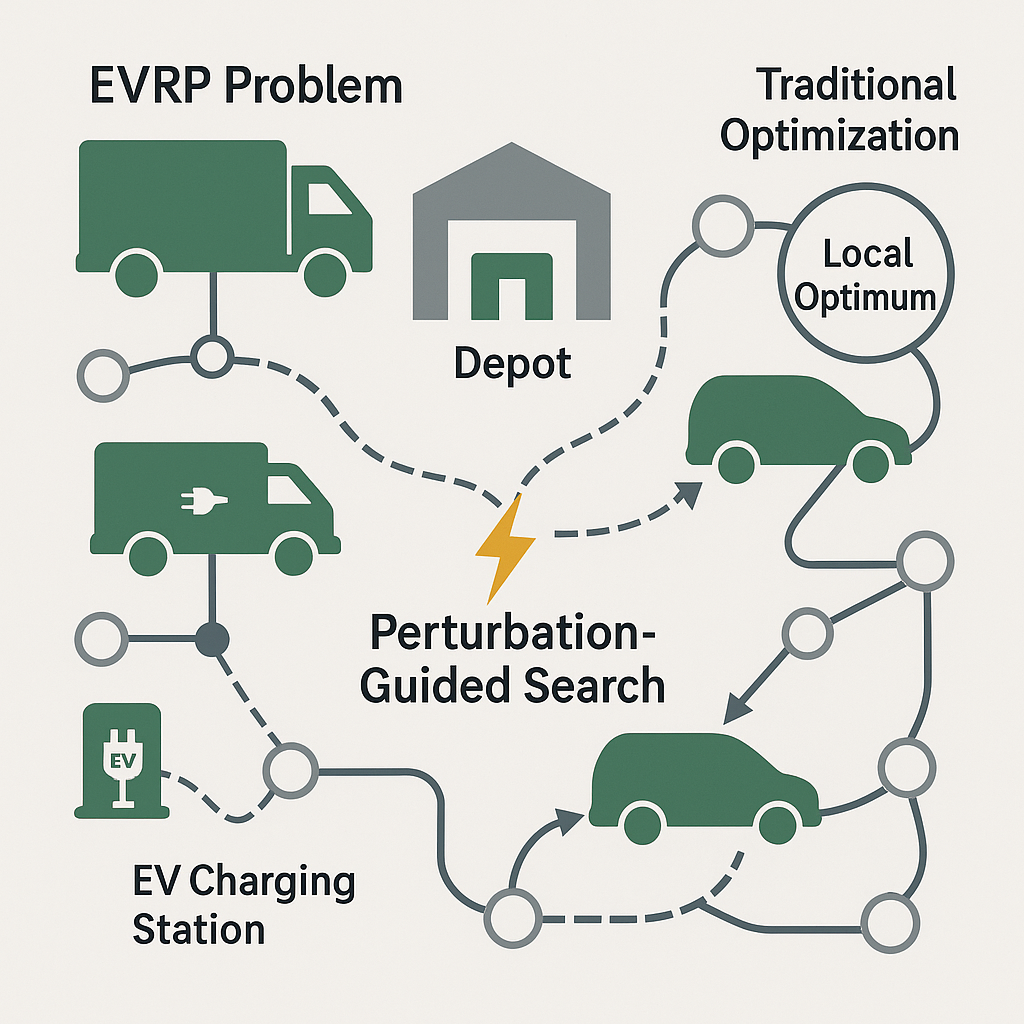
\includegraphics[width=0.8\linewidth]{image/1/main.png}
    \caption{EVRP}
    \label{fig:main}
\end{figure}

The Electric Vehicle Routing Problem (EVRP) (Fig.~\ref{fig:main}), an important extension of the classical Vehicle Routing Problem (VRP), has emerged to address the operational complexities associated with electric vehicle deployments. Unlike the VRP, which focuses solely on minimizing transportation costs under spatial and load constraints, EVRP integrates additional energy-aware considerations, including energy consumption modeling based on distance and payload, battery state-of-charge tracking, mid-route charging decisions, and strategic selection of charging stations~\cite{keskin2016partial, schiffer2017electric, schneider2014electric}.

These enhancements are essential because the deployment of EVs in logistics remains constrained by limited driving range, prolonged charging times, significant battery degradation costs, and sparse charging infrastructure~\cite{nagy2007location}. Traditional VRP models, which assume virtually unlimited range and instantaneous refueling, are therefore insufficient for planning efficient EV-based logistics operations.

To overcome these challenges, EVRP research has advanced along four key dimensions: (i) management and placement of charging stations, (ii) adoption of partial and full recharging strategies, (iii) modeling of nonlinear charging behaviors, and (iv) accommodation of heterogeneous charging station types. Efficiently solving EVRP is critical for enabling scalable and sustainable urban logistics. A feasible solution must simultaneously satisfy customer demands within tight time windows and manage dynamic battery depletion, station availability, and the complex interplay between energy consumption, route topology, and vehicle characteristics. These intertwined constraints render EVRP a highly complex, non-convex, and NP-hard problem, posing significant challenges to exact optimization methods.


\section{Motivation}

As discussed in Section~\ref{sec:broad_overview}, the Electric Vehicle Routing Problem (EVRP) presents unique operational challenges, stemming from limited battery capacities, sparse charging infrastructure, and strict payload restrictions. Traditional metaheuristic algorithms, including Genetic Algorithms (GA), Ant Colony Optimization (ACO), and Simulated Annealing (SA), have been widely applied to EVRP. However, these methods often encounter issues such as premature convergence and limited resilience in recovering from infeasible solutions.

A recent study introduced a clustering-inspired Greedy Search (GS) strategy that aims to address some of these challenges~\cite{hien2023greedy}. By clustering customer paths and greedily selecting charging stations, the GS algorithm produced high-quality initial solutions and, when embedded into a GA framework, demonstrated improved global search effectiveness.

Motivated by these findings, this project seeks to systematically extend the application of structured perturbation strategies to other metaheuristic frameworks, particularly SA and ACO. By integrating perturbation-driven diversification and domain-specific repair mechanisms, we aim to enhance these algorithms' abilities to escape local optima, maintain solution feasibility, and improve overall search robustness. This exploration not only validates the versatility of perturbation techniques across different optimization paradigms but also offers new insights into advancing EVRP solution methodologies.


\section{Aim and Objectives}

\noindent
\paragraph{Aim:}  
The aim of this project is to develop a unified perturbation-driven metaheuristic framework for solving the EVRP under energy and capacity constraints.  
By systematically integrating structured perturbation mechanisms into GA, SA, and ACO, the project seeks to enhance search diversity, improve solution robustness, and enable scalable, energy-aware urban logistics planning.

\bigskip
\noindent
\paragraph{Objectives:}
\begin{enumerate}
    \item \textbf{Conduct a comprehensive literature review:} Analyze and synthesize existing research on metaheuristic approaches for EVRP, with particular focus on the impact of perturbation strategies.
    
    \item \textbf{Implement baseline algorithms:} Develop baseline versions of GA, SA, and ACO adapted to EVRP, ensuring effective handling of energy and load constraints.
    
    \item \textbf{Design structured perturbation mechanisms:} Integrate perturbation-driven diversification into SA and ACO, leveraging insights from GA implementations, to enhance exploration and exploitation balance.
    
    \item \textbf{Develop domain-specific repair and local search strategies:} Incorporate targeted repair methods and multi-stage local search to strengthen solution feasibility and optimize route quality.
    
    \item \textbf{Perform systematic comparative experiments:} Evaluate the performance of perturbation-enhanced algorithms against baseline versions on standard EVRP benchmark datasets, measuring solution quality, computational efficiency, and robustness across multiple runs.
    
    \item \textbf{Assess scalability across problem sizes:} Test and analyze algorithm performance on both small- and large-scale EVRP instances drawn from the WCCI 2020 EVRP Competition benchmark set.
\end{enumerate}

\section{Report Structure}

The remainder of this report is organized as follows:

\begin{figure}[!h]
    \centering
    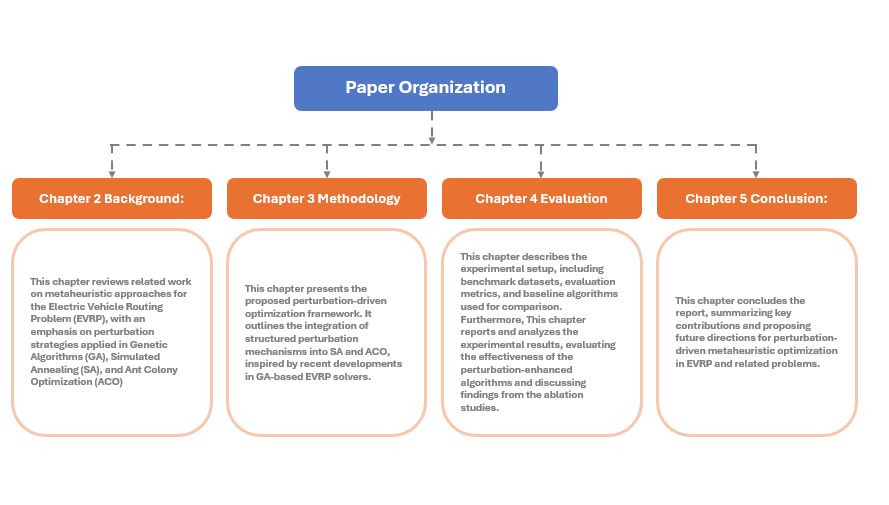
\includegraphics[width=0.8\linewidth]{image/1/paper_structure1.png}
    \caption{Paper's Structure}
    \label{fig:enter-label}
\end{figure}